\section{Comparison between CMA-ES and CE}

\subsection{Global comparison settings}
In all papers used for reference we haven't seen any experiments with different population
and offspring sizes presented side-by-side. However, in our upcoming experimental settings
CMA and CE are most likely to have different population and offspring sizes, which means
that we can't compare them based on iterations/generations. Instead, using the  
\textit{number of agents} as comparison reference, equal terms are secured for both algorithms 
in regards to learning potential. As one of the adjustments to the algorithms are tuning the 
population size, it's required that the frame of reference is invariant.\\
Regarding the graphs themselves, the comparison graphs' x-axis shows the total number 
of Tetris games evaluated, $\sum_{i = 1}^{\generation} \populationSize$. Meanwhile
the y-axis still represents the mean agent's score of the iteration $\generation$.

\subsection{Initial comparison - Bertsekas}
For the initial comparison we use the Bertsekas featureset, since the same featureset
was used for verifying the Cross Entropy implementation. Furthermore, others researchers
has used the Bertsekas featureset as a benchmarking standpoint \citep{thiery:09} \&
\citep{szita:06}.\\
The goal of this comparison is to get an initial idea of how the Shark implementation of
CMA compares to Cross Entropy.\\

\textbf{Results}

\comment{- More statistical results, multilevel model, etc.}\\

Using Cross Entropy with the constant noise setting and CMA with an initial step-size
of $0.5$, we get the following results, seen in figure \ref{fig:CMA_VS_CE_00}.\\

\begin{figure}[H]
\begin{tikzpicture}
\cmaCePlot
\end{tikzpicture}
\caption{Initial comparison between CMA-ES and Cross Entropy \label{fig:CMA_VS_CE_00}}
\end{figure}

As it can be observed in figure \ref{fig:CMA_VS_CE_00} CMA converges faster,
but seems to reach a local optimum around 2,000 agents evaluated. Meanwhile CE has a 
slower convergence but reaches a better local optimum compared to CMA, around 5,500
agents evaluated. In detail CMA on average reaches a score 50,000 rows, and
CE reaches a score of 100,000.\\

\textbf{Analysis and discussion}

These results clearly defy our initial hypothesis, namely we estimated that
CMA would clearly outperform CE, due to CMA's more sophisticated method of 
searching. One reason for this outcome could possible be that
CMA has a very little population size compared to Cross Entropy,
which could be a decisive lack as the evaluation function is non-deterministic with 
a very high variance. These results could indicate that we need to tweak the CMA
configuration, as the CMA local optimum is reached quickly compared to Cross Entropy.
More specifically we might need to adjust the number games played gamer per agent,
since the low population size and increasing variance makes the CMA converge on a
local optimum. But as it can be seen in figure \ref{fig:CMA_VS_CE_00}, the
fast convergence suggests that one game per agent is sufficient until the
score begins to stall at around 1,000-2,000 agents evaluated. It would seem that 
as the CMA-ES reaches a score of around 50,000, variance of the objective function 
appears to render the algorithm incapable of effectively distinguish performance 
of agents. Therefore, to increase the perception of the agents’ performs, 
more evaluations per agent could be necessary at higher scores.\\
\\
As no experiment so far has yielded consistent scores of more than around 200,000 
on average, one explanation could be that the feature set itself poses a limit for 
the optimization algorithms. To address this issue, further experiments will include 
other feature sets. Also, the specific task is not to find a good controller for Tetris, 
but to compare how well each algorithm performs. To reduce runtimes, the Tetris games 
played can be configured to be harder to play. This includes possible reduction of 
board size and posing higher chances of occurrence of pieces that are difficult to place.\\
\\
Therefore, based on the current results, conducting more experiments to discover optimal
settings for CMA-ES seems appropriate.

\subsection{Comparison of featuresets}

The best configurations of the experiments using the Bertsekas
featureset never appears to score much higher than 200,000 lines
on average. Due to this, the question of whether the specific featureset
is the cause of too rapid convergence. To address this, both CMA-ES and Cross
Entropy experiments were run 30 times with respectively the Bertsekas and 
Dellacherie featureset. To prevent long runtimes, the games were simulated
using a harder version of Tetris referred to as 'Hard Tetris'. Regular 
Tetris, all pieces occur with equal likelihood (see figure \ref{fig:TetrisPieces}). To increase the difficulty of the game,
in our hard Tetris, the s-block and z-block appear twice as often 
as the other pieces.

\begin{figure}[H]
\begin{center}
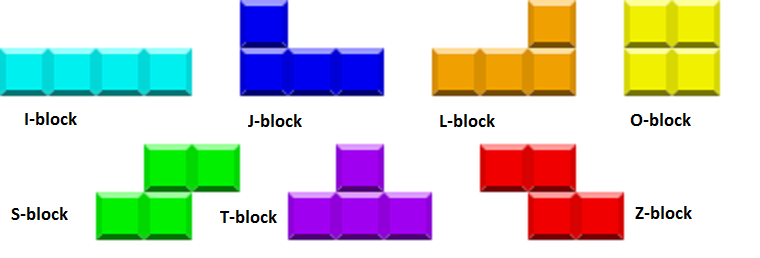
\includegraphics[scale=0.6]{img/Pieces}
\end{center}
\caption{Regular Tetris pieces \label{fig:TetrisPieces}}
\end{figure}



\textbf{Results}

In following figures the mean results of 30 runs of both CMA and Cross 
Entropy is presented. The settings for Cross Entropy remains at constant noise
with a noise term of $z_t = 4$ and an initial sigma of $\sigma_0 = 100.$, 
and the CMA with $\sigma_0 = 1$.\\
\\
Figure \ref{fig:featuresetCompareBertsekas} shows the experiment with the 
Bertsekas featureset. This shows that when running the algorithms with a
harder game, the algorithms behave mostly the same as with regular 
Tetris. Namely that CMA converges faster than Cross Entropy, 
but is eventually outperformed.

\begin{figure}[H]
\begin{tikzpicture}
\plotBertsekasCmaVsCEHardTetris
\end{tikzpicture}
\caption{Comparison between CMA-ES and Cross Entropy 
using hard Tetris and the Bertsekas featureset 
\label{fig:featuresetCompareBertsekas}}
\end{figure}

When using the Dellacherie featureset a similar behaviour is observed.
However, the convergence seems to occur earlier and with a higher score
(figure \ref{fig:featuresetCompareDellacherie}).

\begin{figure}[H]
\begin{tikzpicture}
\plotDellCmaVsCEHardTetris
\end{tikzpicture}
\caption{Comparison between CMA-ES and Cross Entropy 
using hard Tetris and the Dellacherie featureset
\label{fig:featuresetCompareDellacherie}}
\end{figure}

\comment
{
Add full data graphs as appendix.
}



\textbf{Analysis and discussion}

The experiment with different featuresets indicates that the behaviour 
is not heavily dependant on featureset, as the development of the 
graphs closely resemble that from the initial comparison experiment.
Furthermore, it appears that increasing the difficulty of the game
simple shifts the score, but does not affect the development of the graphs.
Therefore, we conclude that changing the featureset does not invalidate
the comparison of the two optimization algorithms.
\comment{
We will also consider it valid to simulate using the faster
hard Tetris when comparing CMA against Cross Entropy.
}

\subsection{Configuration of CMA}
\begin{itemize}
\item Tidligere eksperimenter viser at vi bør justere på cma således det passer bedre til Tetris problemet/featuresættet (population size/offspring regulering, number of games pr agent, nævne at vi benytter hard tetris til eksperimenterne)
\item beskrivelse af eksperiment setup og forventet udfald (begrundelse for hvorfor eksperimenterne udføres)
\item resultater af eksperimenter (grafer, tabeller)
\item analyse og diskussion af resultater
\end{itemize}

In previous sections we focused on tuning Cross Entropy for the Tetris 
problem. Whereas we deliberately chose not to tune CMA due to its implementation 
into the Shark library \citep{shark08}. However, experiments with the "out of 
the box" CMA from Shark, with default settings vs the tuned Cross Entropy
resulted in CMA reaching convergence very fast but not achieving the same point
limit as Cross Entropy.\\
By adjusting the population size to that similar of Cross Entropy, we are able
to get a fair comparison between the two algorithms, given each generation will
contain the same number of agents. By setting the population and offspring size
to the same values, we in effect test if the covariance matrix and the step-size
control has a impact on the algorithm performance compared to Cross Entropy
which does not have the features.\\
Furthermore, CMA also has a unique formula for calculating the updated mean,
called the 'Recombination type' \ref{sec:CMA-ES}. Where the recombination type
determines how much influence each of the offspring vectors has on the next
generation. Built into the CMA algorithm is three methods of recombination. 
\begin{itemize}
\item EQUAL, Each of the offspring vectors has equal influence in the generated mean. Each has $w_i = 1$.
\item LINEAR, The best of the offspring vectors has more influence. 
\item SUPERLINEAR, The vectors are weighted with a logarithmic equation. $w_i = \frac{w_i'}{\sum_{j=1}^{\mu} w_j'^+}$
\end{itemize}
As default, CMA uses Super Linear recombination. However, Tetris is a problem
with multiple local optimums in its solution space. This means, though a vector may be the best in its generation, it could be a nearby local optimum. Therefore, Super Linear recombination may not be the optimal recombination type for the Tetris problem.\\
\\
\comment{Was about to list the experiment setup (population/offspring with recombination type - wait for Oswin conversation to end), will perform experiments with hard tetris}\\
\\
\comment{Reference to CMA-ES section needs to be fixed}\\
\comment{Weights for recombination could have a symbol? (change policy weight
symbol?)}\\
\comment{Find Linear combination type formula of change format of itemize list}

\textbf{Results}

\textbf{Analysis and discussion}


\subsection{Dynamic games played per agent}

\comment{Indledenede tekst}

\textbf{Results}

\comment{- WHAT results did the comparison yield}\\
\comment{- Show results from comparison experiments}


\textbf{Analysis and discussion}

\comment{- WHY did we get these results}\\
\comment{- Discuss the results of the comparison experiments}
